% Tikz File '222tensor.tex'
\documentclass{standalone}
\usepackage{tikz}
%\usetikzlibrary{...}
\begin{document}
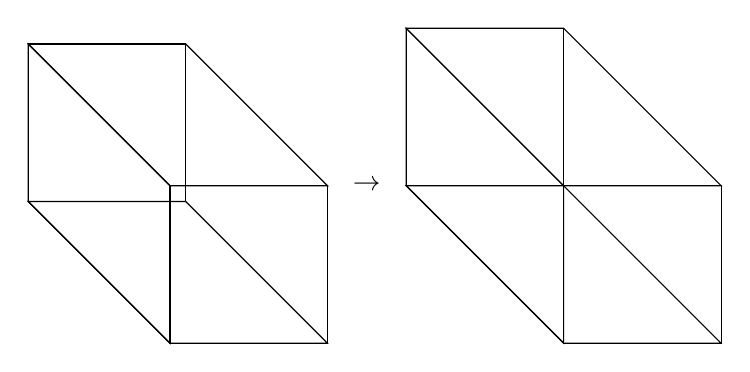
\begin{tikzpicture}  

\def \eps{1.8};

\coordinate (A) at (+2,-2);
\coordinate (B) at (2,0);
\coordinate (C) at (0,0);
\coordinate (D) at (0,-2);

\coordinate (X) at (2-\eps,-2+\eps);
\coordinate (Y) at (2-\eps,0+\eps);
\coordinate (Z) at (0-\eps,0+\eps);
\coordinate (W) at (0-\eps,-2+\eps);

\node at (2.5,0) {$\to$};	

\draw % [very thick, color=blue, fill=green, fill opacity=0.2]
(A) -- (B) -- (C) -- (D) -- cycle;

\draw %[very thick, color=blue, fill=green, fill opacity=0.2]
(X) -- (Y) -- (Z) -- (W) -- cycle;

\draw %[very thick, color=blue, fill=green, fill opacity=0.2]
(B) -- (Y) -- (Z) -- (C) -- cycle;

\draw %[very thick, color=blue, fill=green, fill opacity=0.2]
(C) -- (Z) -- (W) -- (D) -- cycle;

\draw% [very thick, color=blue, fill=green, fill opacity=0.2]
(W) -- (D) -- (A) -- (X) -- cycle;

\coordinate (AA) at (+7,-2);
\coordinate (BB) at (7,0);
\coordinate (CC) at (5,0);
\coordinate (DD) at (5,-2);
\def \eps{2};
\coordinate (XX) at (7-\eps,-2+\eps);
\coordinate (YY) at (7-\eps,0+\eps);
\coordinate (ZZ) at (5-\eps,0+\eps);
\coordinate (WW) at (5-\eps,-2+\eps);

\draw % [very thick, color=blue, fill=green, fill opacity=0.2]
(AA) -- (BB) -- (CC) -- (DD) -- cycle;
\draw %[very thick, color=blue, fill=green, fill opacity=0.2]
(XX) -- (YY) -- (ZZ) -- (WW) -- cycle;
\draw %[very thick, color=blue, fill=green, fill opacity=0.2]
(BB) -- (YY) -- (ZZ) -- (CC) -- cycle;
\draw %[very thick, color=blue, fill=green, fill opacity=0.2]
(CC) -- (ZZ) -- (WW) -- (DD) -- cycle;
\draw% [very thick, color=blue, fill=green, fill opacity=0.2]
(WW) -- (DD) -- (AA) -- (XX) -- cycle;

\end{tikzpicture}
\end{document}